\documentclass[dvisvgm,tikz,border=4pt]{standalone}
\usepackage{amsmath,amssymb}
\usepackage{pgfplots}\pgfplotsset{compat=1.18}\usepgfplotslibrary{polar}
\usetikzlibrary{arrows.meta,positioning,automata,shapes,shapes.misc,calc,decorations.pathmorphing,decorations.markings,angles,quotes,patterns,mindmap,matrix,knots,hobby,trees}
\tikzset{->-/.style={decoration={markings, mark=at position 0.5 with {\arrow{Stealth}}}, postaction={decorate}}}
\begin{document}
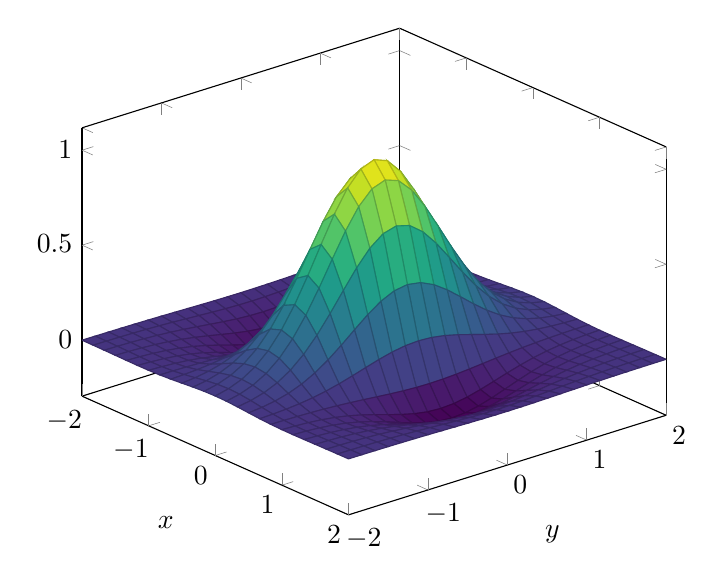
\begin{tikzpicture}
\begin{axis}[view={50}{30}, colormap/viridis, width=9cm, xlabel=$x$, ylabel=$y$]
\addplot3[surf, domain=-2:2, samples=25] {exp(-x^2-y^2)*cos(deg(2*x))};
\end{axis}
\end{tikzpicture}
\end{document}
